\section{am::lambda::binder3$<$ R, P1, P2, P3, A1, A2, A3 $>$ Struct Template Reference}
\label{structam_1_1lambda_1_1binder3}\index{am::lambda::binder3@{am::lambda::binder3}}
{\tt \#include $<$lambda.hpp$>$}

Inherits {\bf am::lambda::detail::lambda\_\-op\_\-tag}.

Inheritance diagram for am::lambda::binder3$<$ R, P1, P2, P3, A1, A2, A3 $>$:\begin{figure}[H]
\begin{center}
\leavevmode
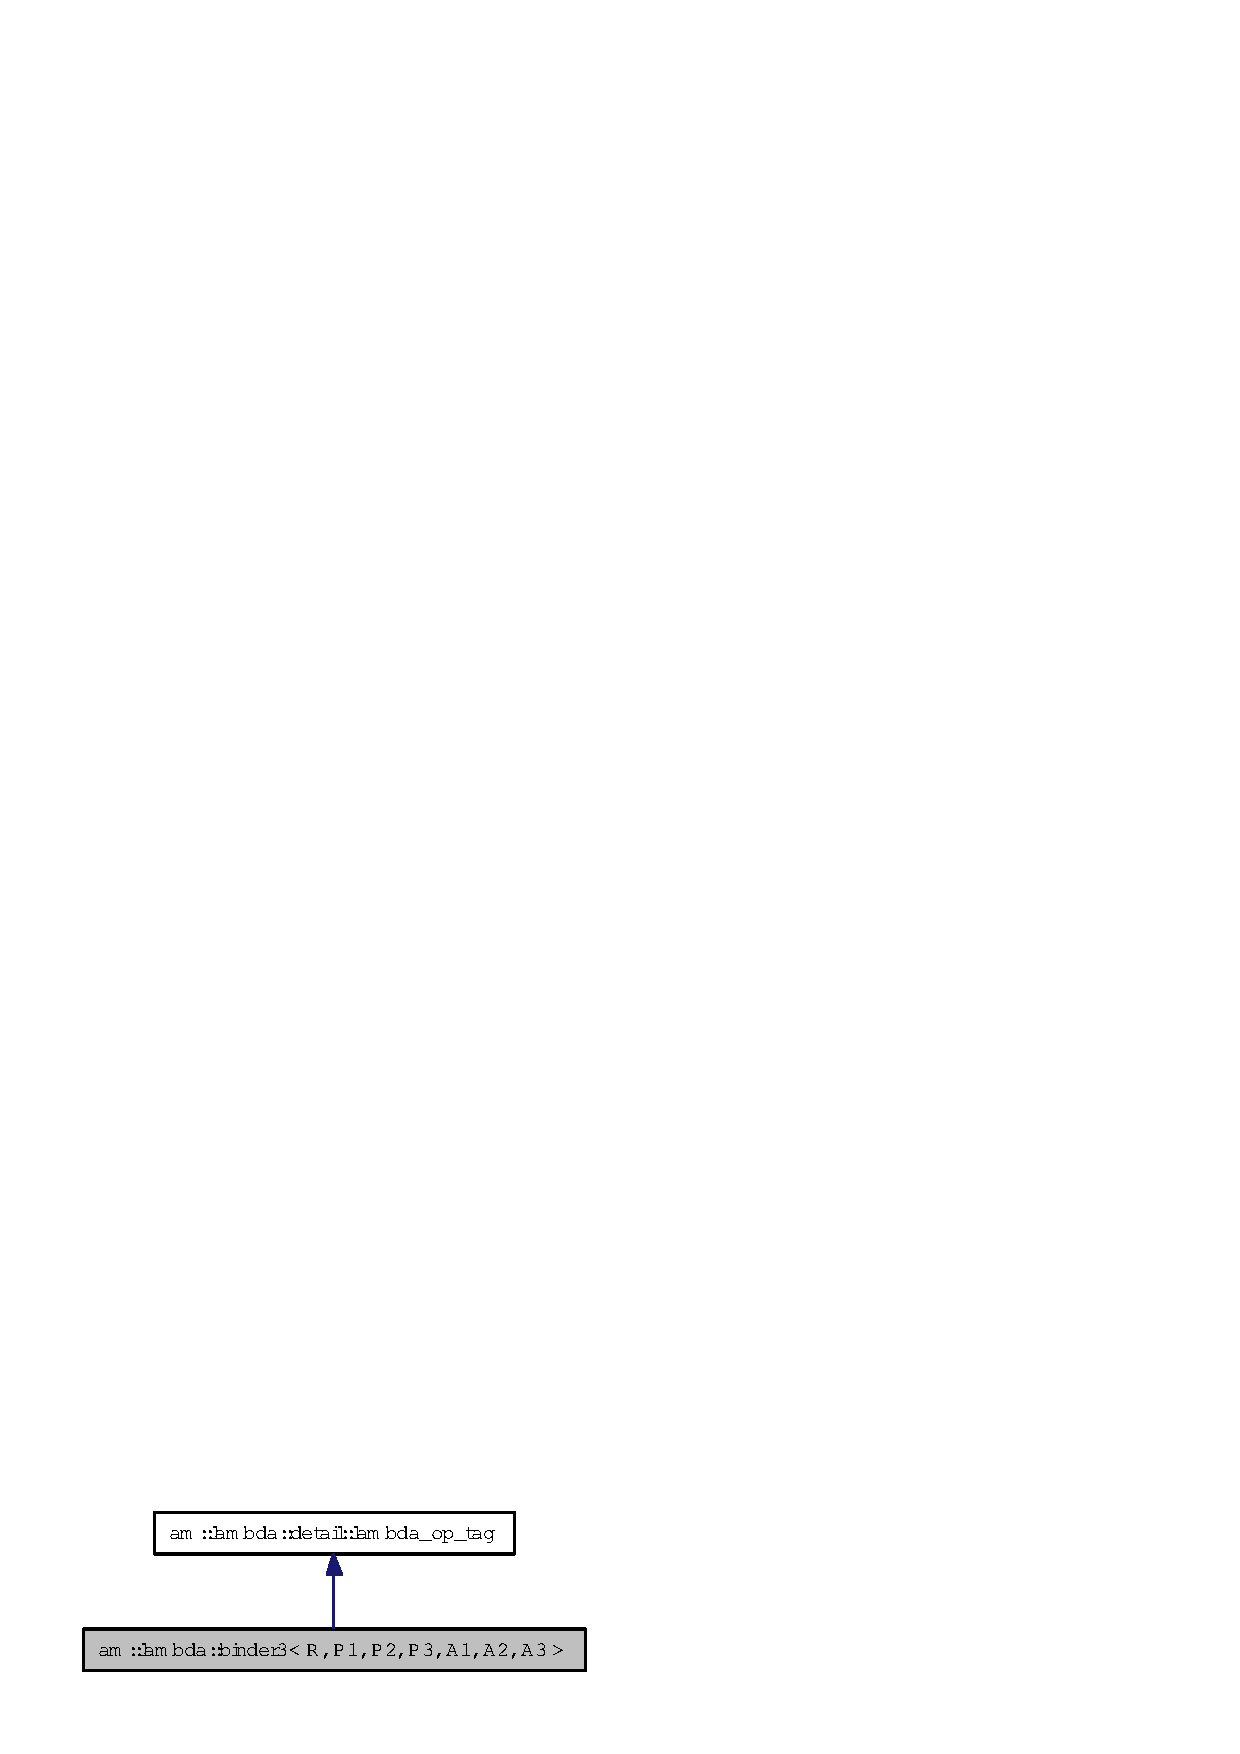
\includegraphics[width=142pt]{structam_1_1lambda_1_1binder3__inherit__graph}
\end{center}
\end{figure}
Collaboration diagram for am::lambda::binder3$<$ R, P1, P2, P3, A1, A2, A3 $>$:\begin{figure}[H]
\begin{center}
\leavevmode
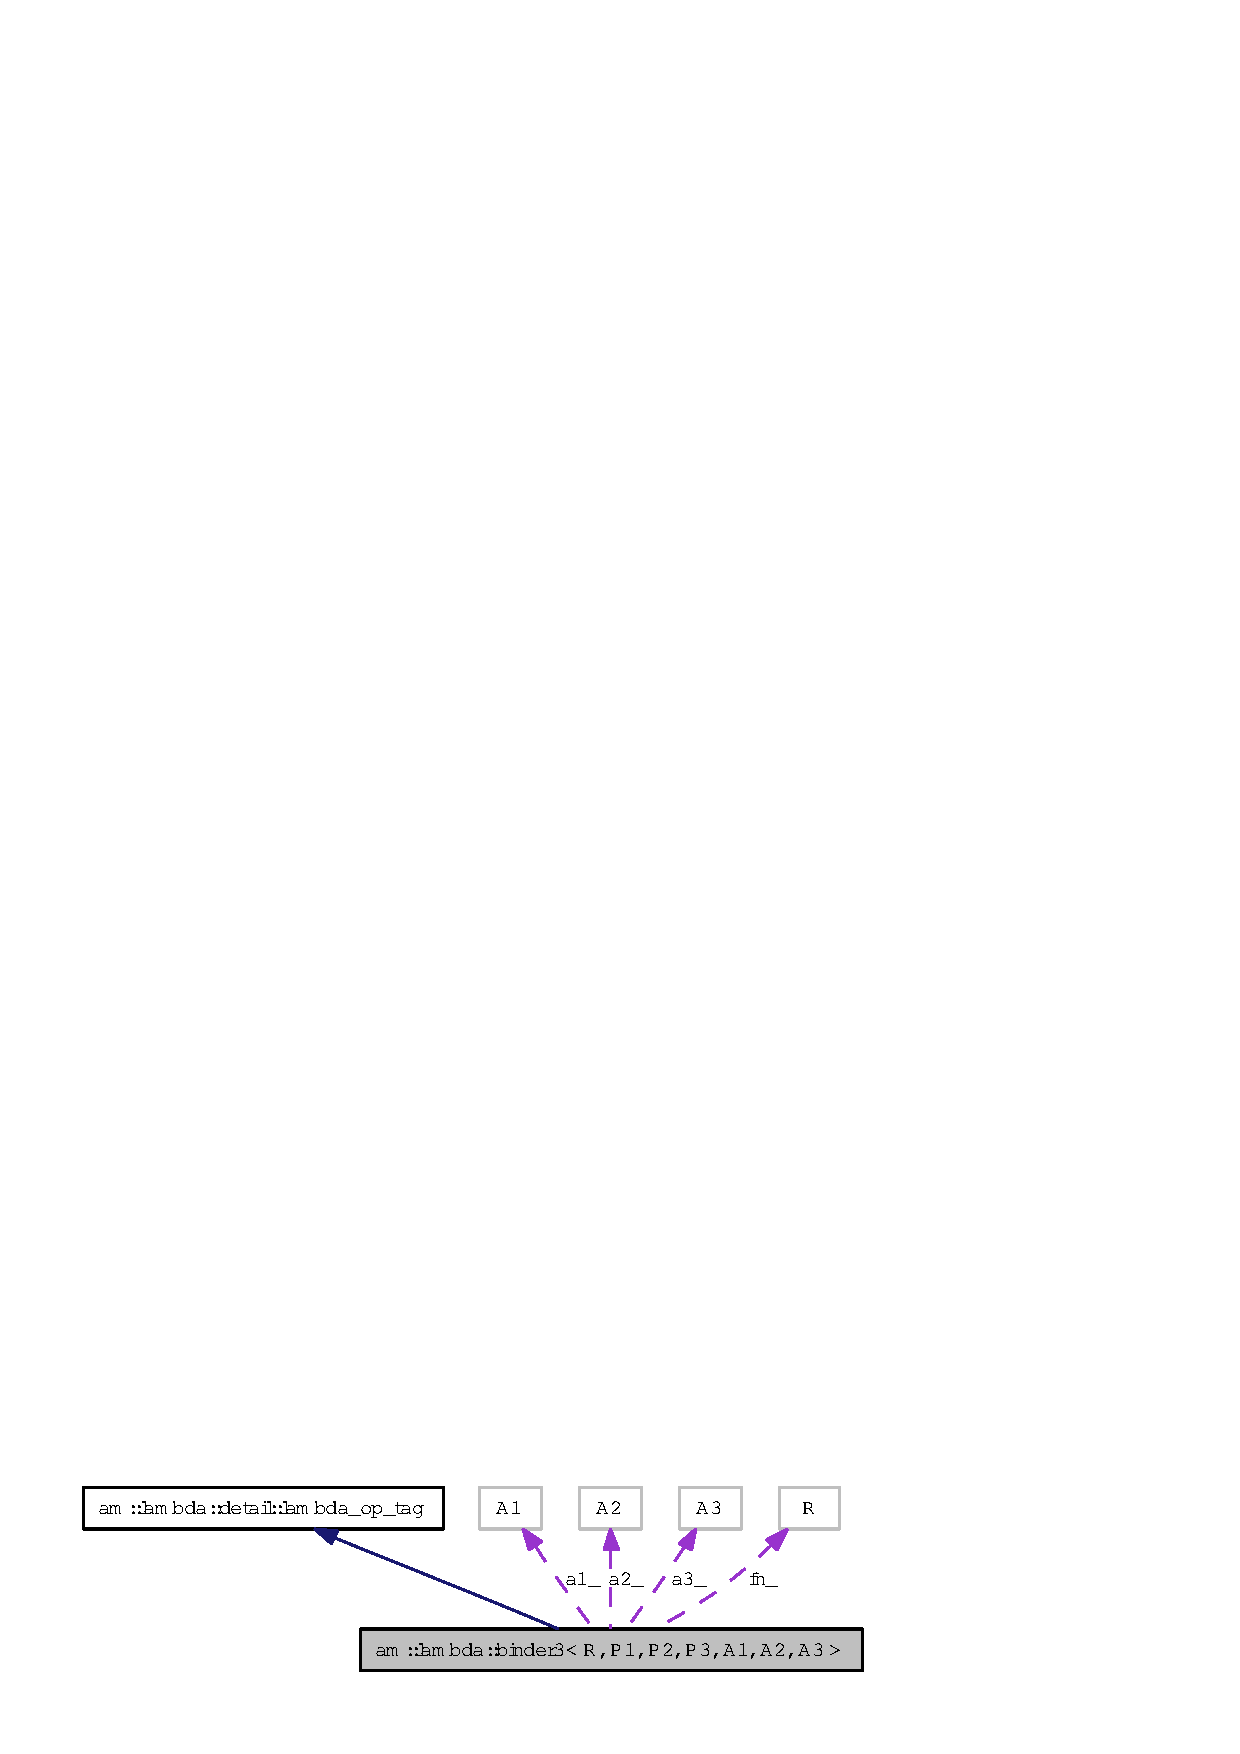
\includegraphics[width=208pt]{structam_1_1lambda_1_1binder3__coll__graph}
\end{center}
\end{figure}
\subsection*{Public Types}
\begin{CompactItemize}
\item 
typedef detail::binder\_\-impl$<$ R $>$::result\_\-type \textbf{result\_\-type}\label{structam_1_1lambda_1_1binder3_4cbe90e647efd7989dedefd02c6d4942}

\end{CompactItemize}
\subsection*{Public Member Functions}
\begin{CompactItemize}
\item 
\textbf{binder3} (R($\ast$fn)(P1, P2, P3), A1 a1, A2 a2, A3 a3)\label{structam_1_1lambda_1_1binder3_0fc64e182ce14a2e0226c4aed7669595}

\item 
template$<$class T1, class T2, class T3$>$ result\_\-type \textbf{operator()} (T1 t1, T2 t2, T3 t3) const \label{structam_1_1lambda_1_1binder3_6e385adbc8d03bb743d036cc66ab5274}

\item 
template$<$class T1, class T2$>$ result\_\-type \textbf{operator()} (T1 t1, T2 t2) const\label{structam_1_1lambda_1_1binder3_2820f406391aee3c5dcaa3698745d2d9}

\item 
template$<$class T1$>$ result\_\-type \textbf{operator()} (T1 t1) const \label{structam_1_1lambda_1_1binder3_88038d1817a18b61ead1ec513ee6e291}

\item 
result\_\-type \textbf{operator()} () const\label{structam_1_1lambda_1_1binder3_6281d09b9414009f2428e22f6b282cb7}

\end{CompactItemize}
\subsection*{Public Attributes}
\begin{CompactItemize}
\item 
R($\ast$ \textbf{fn\_\-} )(P1, P2, P3)\label{structam_1_1lambda_1_1binder3_11ea57f8e411cf238142c8893d59d9c6}

\item 
A1 \textbf{a1\_\-}\label{structam_1_1lambda_1_1binder3_2e578b8d898e9221094c6ef64362aa98}

\item 
A2 \textbf{a2\_\-}\label{structam_1_1lambda_1_1binder3_fcf561d9b972eb387ad91b0c6c605e71}

\item 
A3 \textbf{a3\_\-}\label{structam_1_1lambda_1_1binder3_94d9591a62e2343b0889c57ada1511e0}

\end{CompactItemize}


\subsection{Detailed Description}
\subsubsection*{template$<$typename R, typename P1, typename P2, typename P3, typename A1, typename A2, typename A3$>$ struct am::lambda::binder3$<$ R, P1, P2, P3, A1, A2, A3 $>$}

Binder for the free function which takes three arguments. 



The documentation for this struct was generated from the following file:\begin{CompactItemize}
\item 
{\bf lambda.hpp}\end{CompactItemize}
